\documentclass{article}

\usepackage[brazil]{babel}
\usepackage[latin1,utf8]{inputenc}
\usepackage{pifont}

%% Math
\usepackage{mathtools}
\usepackage{amsmath}
\usepackage{commath}

\usepackage{amsfonts}% revise se precisa ou não
\usepackage{nccmath}% revise se precisa ou não

\usepackage[numbers]{natbib}
\usepackage{multirow}
\usepackage{makecell}
\usepackage{graphicx}

\usepackage{listings}
\usepackage{float}
\usepackage{enumitem}

\usepackage{wasysym}

\renewcommand{\lstlistingname}{Código}
\renewcommand{\lstlistlistingname}{Lista de \lstlistingname s}

%\definecolor{codegreen}{rgb}{0,0.6,0}
%\definecolor{codegray}{rgb}{0.85,0.85,0.85}
%\definecolor{codepurple}{rgb}{0.58,0,0.82}
%\definecolor{codeblack}{rgb}{0,0,0}

\lstdefinelanguage{JavaScript}{
  keywords={typeof, new, true, false, catch, function, return, null, catch, switch, var, if, in, while, do, else, case, break},
  %keywordstyle=\color{blue}\bfseries,
  ndkeywords={class, export, boolean, throw, implements, import, this},
  %ndkeywordstyle=\color{codegray}\bfseries,
  %identifierstyle=\color{black},
  sensitive=false,
  comment=[l]{//},
  morecomment=[s]{/*}{*/},
  %commentstyle=\color{purple}\ttfamily,
  %stringstyle=\color{red}\ttfamily,
  morestring=[b]',
  morestring=[b]"
}

\lstdefinestyle{codigo}{
    backgroundcolor=\color{codegray},   
    commentstyle=\color{codegreen},
    keywordstyle=\color{magenta},
    numberstyle=\tiny\color{codeblack},
    stringstyle=\color{codepurple},
    basicstyle=\ttfamily\footnotesize,
    breakatwhitespace=false,         
    breaklines=true,                 
    captionpos=b,                    
    keepspaces=true,                 
    numbers=left,                    
    numbersep=5pt,                  
    showspaces=false,                
    showstringspaces=false,
    showtabs=false,                  
    tabsize=4
}

\lstset{style=codigo}

\DeclarePairedDelimiter{\round}\lfloor\rceil
\newcommand\citetxt[1]{%
  \citeauthor{#1}~(\citeyear{#1})}
\newcommand\citepar[1]{%
  (\citeauthor{#1}, \citeyear{#1})} 


%https://tex.stackexchange.com/q/151984/7561
\DeclarePairedDelimiterX{\infdivx}[2]{(}{)}{%
  #1\;\delimsize\|\;#2%
}
\newcommand{\kl}{\operatorname{KL}\infdivx}
\newcommand{\skl}{\operatorname{SKL}\infdivx}

% https://tex.stackexchange.com/questions/23773/a-centered-plus-minus-symbol
\newcommand{\rpm}{\raisebox{.2ex}{$\scriptstyle\pm$}}

% https://tex.stackexchange.com/a/141685/7561
\newcommand\givenbase[1][]{\:#1\lvert\:}
\let\given\givenbase

% https://tex.stackexchange.com/a/171959/7561
\newcommand\reallywidehat[1]{\ThisStyle{%
    \setbox0=\hbox{$\SavedStyle#1$}%
    \stackengine{-1.0\ht0+.5pt}{$\SavedStyle#1$}{%
      \stretchto{\scaleto{\SavedStyle\mkern.15mu\char'136}{1.5\wd0}}{1.4\ht0}%
    }{O}{c}{F}{T}{S}%
}}
\newcommand{\hkl}{\widehat{\operatorname{KL}}\infdivx}

% Conditional independence symbol
% https://tex.stackexchange.com/questions/218631/symbol-for-not-conditionally-independent/
\newcommand{\CI}{\mathrel{\perp\mspace{-10mu}\perp}}

% declare my argmin and argmax operators
% https://tex.stackexchange.com/a/5255/7561
\DeclareMathOperator*{\argmax}{arg\,max}
\DeclareMathOperator*{\argmin}{arg\,min}

% declaring an expectation operator to behave like sum
% https://tex.stackexchange.com/a/23436/7561
\makeatletter
\DeclareRobustCommand\bigop[1]{%
  \mathop{\vphantom{\sum}\mathpalette\bigop@{#1}}\slimits@
}
\newcommand{\bigop@}[2]{%
  \vcenter{%
    \sbox\z@{$#1\sum$}%
    \hbox{\resizebox{\ifx#1\displaystyle.9\fi\dimexpr\ht\z@+\dp\z@}{!}{$\m@th#2$}}%
  }%
}
\makeatother

% Keywords command
\providecommand{\keywords}[1]
{
  \small	
  \textbf{\textit{Keywords ---}} #1
}
\providecommand{\palavraschave}[1]
{
  \small	
  \textbf{\textit{Palavras-chave ---}} #1
}

%\newcommand{\E}{\DOTSB\bigop{\mathbb{E}}}
\DeclareMathOperator*{\E}{\mathbb{E}}

% redefining \times operator
\let\oldtimes\times
\def\times{{\mkern1mu\oldtimes\mkern1mu}}



\usepackage{subfigure}
\newcommand{\cmark}{\ding{51}}%

%\DeclarePairedDelimiter\abs{\lvert}{\rvert}%
%\DeclarePairedDelimiter\norm{\lVert}{\rVert}%
\DeclarePairedDelimiter\product{\langle}{\rangle}%

\usepackage{cellspace}
\setlength\cellspacetoplimit{6pt}
\setlength\cellspacebottomlimit{4pt}

%% Units
\usepackage{siunitx}

%% Tables
\usepackage{booktabs}


% Para acrescentar comentários ao PDF descomente:
\usepackage
%  [pdfauthor={nome do autor},
%   pdftitle={titulo},
%   pdfkeywords={palavra-chave, palavra-chave},
%   pdfproducer={Latex with hyperref},
%   pdfcreator={pdflatex}]
{hyperref}

% Os cores podem ser mudados
\hypersetup{
%  linkcolor={red!50!black},
%  citecolor={blue!50!black},
%  urlcolor={blue!80!black}
}

\title{\textit{Workflow} autonômico para aplicações de \textit{Machine Learning} utilizando métricas de \textit{Fairness}}

\author{Thales Eduardo Nazatto\textsuperscript{1}, Cecília Mary Fischer Rubira\textsuperscript{2}, Leonardo Montecchi\textsuperscript{3}}
\date{
	\textsuperscript{1} UNICAMP, Campinas, Brasil, tenazatto@gmail.com
	\\
	\textsuperscript{2} UNICAMP, Campinas, Brasil, cmrubira@ic.unicamp.br
	\\
	\textsuperscript{3} NTNU, Trondheim, Noruega, leonardo.montecchi@ntnu.no\\[2ex]
	\today
}

\begin{document}

\maketitle

\begin{abstract}
O uso de Inteligência Artificial (IA) envolvendo grandes volumes de dados vem crescendo conforme nossa sociedade migra processos manuais de trabalho para soluções digitais e necessita de tomadas de decisão mais rápidas e assertivas, mas, devido a barreiras éticas e legais, métricas usadas inicialmente para definir a eficácia de um algoritmo se mostraram limitadas para medir vieses que refletem a sociedade de maneira que não era esperada pelos desenvolvedores da solução. Para resolver tal problema, novos algoritmos foram desenvolvidos e um novo conjunto de métricas, denominado como métricas de Fairness, é utilizado para determinar um equilíbrio entre grupos que sofrem discriminações. Com a introdução deste novo conjunto de algoritmos e métricas, novos problemas surgem, aumentando a complexidade da análise do Cientista de Dados para obter modelos de forma otimizada. Esta dissertação de Mestrado possui o objetivo de contribuir com o tema de Inteligência Artificial (IA) do ponto de vista da Engenharia de Software, apresentando um \textit{Workflow} para aplicações de \textit{Machine Learning} que pode ser executado de maneira autônoma sem a necessidade de experimentar uma grande quantidade de técnicas e pode ser mais assertivo em encontrar opções mais otimizadas para diferentes contextos. Para isso, é utilizado a arquitetura Pipe-and-Filter para realizar o \textit{Workflow}, utilizando proveniência de dados para gravação de metadados, e a arquitetura MAPE-K para determinar essa autonomia. Foram realizados diversos estudos de caso para determinar se o MAPE-K pode ser viável na resolução destes problemas, e se o \textit{Workflow} pode ser evoluído sem grande complexidade, e foi possível notar que as arquiteturas propostas conseguiram ser robustas e modulares, possibilitando estudos de Engenharia de Software em aplicações com o uso responsável de dados.

\keywords{\textit{Workflow}, \textit{Machine Learning}, Inteligência Artificial, Computação Autônoma, Métricas de \textit{Fairness}}
\end{abstract}

\section{Introdução}

Técnicas de Inteligência Artificial e Aprendizado de Máquina já são utilizadas há bastante tempo no ramo da Computação. Ramos como robótica e jogos são grandes exemplos, dada a necessidade nos mesmos de automatizar comportamentos que seriam tidos como triviais para um ser humano. Entretanto, nos últimos anos ocorreu um crescimento no uso dessas tecnologias em aplicações tradicionais, devido principalmente à grande quantidade de dados processada diariamente pelas empresas e pela quantidade de processamento disponível a custos baixos. Diferentes perfis podem traçados com esses dados e usar soluções de IA gera tomadas de decisão mais assertivas com o objetivo de melhorar a experiência de usuário e corrigir problemas. Porém, muitas dessas soluções foram projetadas sem pensar em governança de dados como requisito de projeto, e se mostram ineficientes quando ela é tratada em consideração. E nesse ponto muitas aplicações de IA falham: muitas implementações foram implementadas como \textit{black boxes}, onde o determinante para estabelecer a confiança no modelo implementado é sua entrada e sua saída.

Um outro efeito colateral dessa estratégia é a exposição de vieses que, embora sejam vistos como não-intencionais pelos desenvolvedores por ter a possibilidade de ser um \textit{outlier} no modelo treinado, refletem preconceitos escancarados da sociedade atual. Uma entrada de dados enviesada resulta em um algoritmo que realiza discriminações em sua classificação~\citep{Buolamwini_2018}, e uma vez que as métricas utilizadas para medir a qualidade de um modelo \textit{black box} são geralmente baseadas em acurácia, precisão e recall, discriminações não são facilmente percebidas por tais métricas. Ao mesmo tempo, um modelo \textit{black box} pode ter uma alta dependência de poucos dados, determinando problemas de acoplamento. Para resolver este problema, é possível que a criação de um novo modelo seja uma melhor opção que realizar a correção em apenas parte dele.

Devido a esses tipos de problemas, o termo \textit{Explainable AI} (XAI) ganha força para envolver o desenvolvimento de uma IA que seja acurada e simultaneamente transparente. Como IA possui diversos tipos de métodos diferentes para enquadrar diversos tipos de dados, o mesmo acaba se aplicando em Explainable AI, podendo enquadrar em diversos tipos de dados~\citep{Sundararajan_2017}, ou dados específicos como imagens~\citep{Kapishnikov_2019} e tabelas~\citep{Maleki_2013}. Como o objetivo em XAI é fazer com que os resultados alcançados pela solução de IA sejam compreendidos por humanos, é possível considerar este fato como requisito no design de uma solução de IA, fazendo com que a mesma seja reusável e testável.

No mesmo tema, é possível estabelecer métricas para determinar o quão o modelo está preparado para dados sensíveis~\citep{Begley_2021}, termo que é conhecido como \textit{Fairness}. Com a evolução das pesquisas na comunidade acadêmica, foram descobertos algoritmos para redução dos vieses presentes nos conjuntos de dados, como \textit{Reweighing}~\citep{Kamiran_2011}, \textit{Adversarial Debiasing}~\citep{Zhang_2018} e \textit{Reject Option Classification}~\citep{Kamiran_2012}. Por consequência, ocorre melhora nas métricas em questão, mas pode desfavorecer métricas que já são amplamente utilizadas como garantia de um bom modelo desenvolvido com técnicas de Aprendizado de Máquina.

O objetivo desta dissertação de mestrado é desenvolver uma estrutura de \textit{Workflow} para aplicações de \textit{Machine Learning} que seja completamente autônoma, por três fatores principais:

\begin{itemize}
\item Facilitar a criação de modelos justos e confiáveis com a automatização da escolha dos algoritmos, cuja complexidade aumenta com a escolha dos algoritmos a serem utilizados e suas execuções nas etapas corretas do processo, onde eles foram escolhidos para atuar.
\item Estabelecer um balanceamento entre métricas para avaliar bons modelos com métricas para avaliar modelos justos.
\item Considerar proveniência de dados como requisito no design de uma solução de IA, e como uma alternativa a XAI através da utilização de metadados.
\end{itemize}

Para isso, foi desenvolvido um sistema, que pode ser dividido em 4 etapas principais: Engenharia de dados, \textit{Workflow} de IA, Autonomia do \textit{Workflow} e Interface Humano-Computador. Para o desenvolvimento do \textit{workflow}, será utilizada a arquitetura \textit{Pipe-and-Filter}. Para a autonomia deste, será criado um componente utilizando a arquitetura MAPE-K~\citep{IBM_2005} para analisar uma base de conhecimento e prover o melhor pipeline seguindo regras pré-determinadas. Para a interface, ela foi criada nos moldes de uma aplicação web. O código deste desenvolvimento foi disponibilizado no GitHub\footnote{Repositório Git contendo os códigos deste projeto: \url{https://github.com/tenazatto/MsC}} para avaliação e testes em estudos posteriores.

O restante deste artigo se organizará da seguinte forma: o Capítulo 2 descreve os conceitos que irão ser abordados neste projeto; o Capítulo 3 mostra a metodologia e detalhamento do processo de desenvolvimento; o Capítulo 4 discute os resultados obtidos e, finalmente, o Capítulo 5 estabelece as conclusões, considerações finais e sugestões de trabalhos futuros e evoluções.

\section{Conceitos Principais}

\subsection{\textit{Machine Learning}}
Aprendizado de Máquina (\textit{Machine Learning}, em inglês) pode ser definido como “a prática de usar algoritmos para coletar dados, aprender com eles, e então fazer uma determinação ou predição sobre alguma coisa no mundo. Então em vez de implementar as rotinas de software manualmente, com um gama específica de instruções para completar uma tarefa em particular, a máquina é `treinada` usando uma quantidade grande de dados e algoritmos que dão e ela a habilidade de aprender como executar a tarefa”~\citep{Copeland_2016}. Com isso, o computador consegue a habilidade de realizar determinado cálculo ou tarefa sem que necessite de programação adicional ou interferência humana para isso.

O \textit{Machine Learning} é fortemente relacionado com a Estatística, uma vez que seus métodos e parte de seus algoritmos, como regressões, tiveram como base modelos estatísticos e a análise de seus dados. As tarefas de aprendizado podem ser classificadas em três categorias básicas~\citep{MLWikipedia_2021}~\citep{MLSAS_2021}:

\begin{itemize}
\item \textbf{Aprendizado supervisionado}: O treinamento é realizado por meio de exemplos rotulados, como uma entrada na qual a saída desejada é conhecida. Através de métodos como classificação, regressão e \textit{gradient boosting}, o aprendizado supervisionado utiliza padrões para prever os valores de rótulos em dados não-rotulados adicionais. O aprendizado supervisionado é comumente empregado em aplicações nas quais dados históricos preveem eventos futuros prováveis.
\item \textbf{Aprendizado não-supervisionado}: É utilizado em dados que não possuem rótulos históricos. A “resposta certa” não é informada ao sistema, o algoritmo deve descobrir o que está sendo mostrado. O objetivo é explorar os dados e encontrar alguma estrutura dentro deles. Técnicas populares incluem mapas auto-organizáveis, mapeamento por proximidade, agrupamento \textit{k-means} e decomposição em valores singulares. Esses algoritmos também são utilizados para segmentar tópicos de texto, recomendar itens e identificar pontos discrepantes nos dados.
\item \textbf{Aprendizado por reforço}: O algoritmo descobre através de testes do tipo “tentativa e erro” quais ações rendem as maiores recompensas. Este tipo de aprendizado possui três componentes principais: o agente (o aprendiz ou tomador de decisão), o ambiente (tudo com que o agente interage) e ações (o que o agente pode fazer). O objetivo é que o agente escolha ações que maximizem a recompensa esperada em um período de tempo determinado. O agente atingirá o objetivo muito mais rápido se seguir uma boa política, então o foco do aprendizado por reforço é descobrir a melhor política.
\end{itemize}

O termo \textit{Machine Learning} se tornou muito mais evidente com a possibilidade da implementação do \textit{Deep Learning}, que é uma técnica que utiliza Redes Neurais Artificiais para atingir seus resultados. Redes Neurais Artificiais são modelos computacionais inspirados no sistema nervoso do cérebro, onde temos neurônios divididos em camadas e conectados entre si, podendo ser abstraído conforme ilustração na Figura \ref{fig:NeuralNetwork}. Dependendo da tarefa a ser realizada, cada neurônio atribui um peso para os dados que entram e a saída final é determinada pelo total desses pesos~\citep{Copeland_2016}. As redes neurais utilizadas em \textit{Deep Learning} possuem, ao menos, duas camadas de neurônios entre a camada que recebe os dados de entrada e a camada final que faz o tratamento final dos dados de saída.

\begin{figure}[H]
\centering
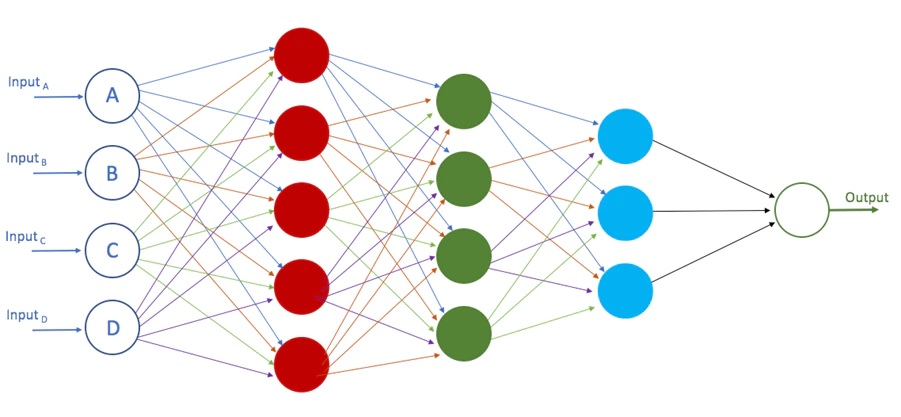
\includegraphics[scale=0.8]{images/deep_neural_network.jpg}
\caption {Exemplo de uma rede neural utilizada em \textit{Deep Learning}.}
\label{fig:NeuralNetwork}
\end{figure}

Com a evolução da computação, o treino de uma tarefa passou a ser cada vez mais viável, uma vez que a execução de algoritmos de \textit{Machine Learning} é computacionalmente muito custosa, especialmente quando redes neurais são utilizadas. E sua viabilidade é acompanhada de efetividade: Como exemplo, reconhecimento de imagens por máquinas treinadas através de deep learning em alguns cenários possuem uma taxa de acerto maior que a de humanos~\citep{Copeland_2016}.
\subsection{\textit{Fairness} em \textit{Machine Learning}}

Com o aumento do uso de \textit{Machine Learning} para tomadas de decisão, o uso de dados sensíveis em um contexto determinado também aumentou, e temas como uma IA ética e conceitos como vieses nos dados e \textit{Fairness} passaram a serem discutidas não apenas na Computação, mas em áreas como Direito. Algoritmos são mais objetivos, rápidos e são capazes de considerar uma grande magnitude de recursos que pessoas não são capazes. Entretanto, até o presente momento eles não são capazes de diferenciar contextos sociais, onde um resultado mais eficiente de acordo com os dados disponíveis podem amplificar as desigualdades sociais e tomar decisões de modo injusto~\citep{Mehrabi_2021}. 

Estes dados sensíveis, tendo como exemplos cor de pele, raça, sexo, idade e altura, são considerados atributos protegidos, que precisam ser classificados e processados antes da execução de um algoritmo de \textit{Machine Learning}, determinarão como o algoritmo se comportará e, consequentemente, afetará suas métricas~\citep{Mougan_2022}. Os grupos de dados provenientes destes atributos protegidos são considerados grupos protegidos, que podem ser divididos em dois grupos: o grupo privilegiado, que possui vantagens no contexto do problema, e o grupo não-privilegiado, que possui desvantagens no contexto do problema e, portanto, sujeito a discriminação.

É possível descrever o conceito de \textit{Fairness} no contexto de aprendizagem supervisionada, onde um modelo $f$ pode prever um conjunto de resultados $y$ a partir de um conjunto de \textit{features} $x$, evitando discriminação injusta em relação a um atributo protegido $a$. É permitido, mas não exigido, que $a$ seja um componente de $x$~\citep{Begley_2021}. Em outras palavras, um modelo de ML considerado justo é aquele onde a correlação de seu resultado é baixa em relação a dados de entrada considerados como sensíveis a discriminações.

Para avaliar a justiça de um modelo, as métricas utilizadas diferem das métricas utilizadas para avaliação do modelo, que possuem o propósito de verificar se um modelo tem previsões confiáveis ou não. As métricas de \textit{Fairness} possuem um propósito diferente, pois verificam os dados de forma mais intimista. Elas não medem o modelo como um todo, mas o quanto os grupos e registros avaliados estão próximos dos outros. Enquanto as métricas mais tradicionais avaliam a performance do modelo e seus dados como um todo e seus resultados gerais, as métricas de \textit{Fairness} avaliam se os resultados gerais também se refletem em grupos específicos, para verificar se não há disparidade ou discriminação nos resultados propostos.

Exemplos de métricas utilizadas para isso são a Taxa de Verdadeiros Positivos e a Taxa de Falsos Positivos. Enquanto a \textbf{Taxa de Verdadeiros Positivos} (TVP, ou TPR pelo termo em inglês \textbf{True Positive Rate}) é a fração de casos positivos reais (TP) de todos os casos negativos previstos incorretamente como estando na classe positiva (FN), a \textbf{Taxa de Falsos Positivos} (TFP, ou FPR pelo termo em inglês \textbf{False Positive Rate}) é a fração de casos negativos previstos incorretamente como estando na classe positiva (FP) de todos os casos positivos reais (TN):

\begin{equation}
TPR = \frac{TP}{TP + FN}
FPR = \frac{FP}{FP + TN}
\end{equation}

Dada essas métricas iniciais, considerando $Y=1$ a classe positiva, $Z=0$ o grupo não-privilegiado e $Z=1$ o grupo privilegiado, algumas das definições de \textit{Fairness} mais usadas são as seguintes:

\begin{itemize}
\item \textbf{Diferença de paridade estatística (\textit{Statistical parity difference}), ou discriminação~\citep{Zemel_2013}:} Esta métrica é baseada na seguinte fórmula:

\begin{equation}
Pr(Y=1|Z=0)-Pr(Y=1|Z=1)
\end{equation}
 
Aqui, o viés ou paridade estatística é a diferença entre a probabilidade de que um indivíduo aleatório retirado dos não-privilegiados seja rotulado como 1 e a probabilidade de que um indivíduo aleatório dos privilegiados seja rotulado como 1. Portanto, um valor próximo de 0 é considerado justo.

\item \textbf{Diferença de oportunidade igual (\textit{Equal opportunity difference})~\citep{Biswas_2020}:} É a diferença entre a taxa positiva verdadeira do grupo não privilegiado e a taxa positiva verdadeira do grupo privilegiado:

\begin{equation}
TPR_{Z=0} - TPR_{Z=1}
\end{equation}
 
Um valor próximo de 0 é considerado justo. Um classificador binário satisfaz a igualdade de oportunidades quando a taxa positiva verdadeira de ambos os grupos são iguais~\citep{Hardt_2016}

\item \textbf{Diferença de probabilidade média (\textit{Average odds difference})~\citep{Biswas_2020}:} Essa métrica usa a taxa de falsos positivos e a taxa positiva verdadeira para calcular a tendência, calculando a igualdade de probabilidades com a fórmula:

\begin{equation}
\frac{1}{2}(|FPR_{Z=0} - FPR_{Z=1}|+|TPR_{Z=0} - TPR_{Z=1}|)
\end{equation}
 
Precisa ser próximo a 0 para ser considerado justo.

\item \textbf{Impacto de disparidade (\textit{Disparate impact})~\citep{Biswas_2020}:} Para esta métrica, é usada a seguinte fórmula:

\begin{align*}
\frac{Pr(Y=1|Z=0)}{Pr(Y=1|Z=1)}
\end{align*}

Usa as mesmas probabilidades da diferença de paridade estatística, mas aqui são calculadas como proporção. Desta forma, um valor próximo de 1 é considerado justo.

\item \textbf{Índice de Theil (\textit{Theil index})~\citep{Speicher_2018}:} Esta medida também é conhecida como índice de entropia generalizado, mas com $\alpha$ igual a 1~\citep{Speicher_2018}. É calculado com a seguinte fórmula:

\begin{align*}
\frac{1}{n}\sum^{n}_{i=0}\frac{b_i}{\mu}\ln{\frac{b_i}{\mu}}
\end{align*}

Onde $b_i = \hat{y}_i - y_i + 1$, $y_i$ é o conjunto de saídas e $\hat{y}_i$ é o conjunto de previsões dadas pelo modelo. Também precisa ser próximo a 0 para ser considerado justo.

\end{itemize}

\subsection{Computação Autônoma}

Em 2001, Paul Horn introduziu o conceito de Computação Autônoma como alternativa a solução para a crescente complexidade dos sistemas da época, onde previa-se que os mesmos se tornariam muito grandes e complexos até mesmo para os profissionais mais qualificados configurarem e realizarem manutenção. Tal conceito qualifica sistemas de computação que podem se autogerenciar com relação aos objetivos de alto nível dados pelos administradores e é derivado da biologia, dado a grande variedade e hierarquia de sistemas autônomos presentes na natureza e na sociedade~\citep{Kephart_2003}. 

Em um ambiente autônomo e autogerenciado, os componentes de sistema podem incorporar como funcionalidade um \textit{loop} de controle. Embora estes \textit{loops} sejam divididos nos mesmos procedimentos, é possível categorizá-los em 4 categorias principais. Essas categorias são consideradas atributos dos componentes do sistema e são definidas como~\citep{IBM_2005}:

\begin{itemize}
\item \textbf{Auto-configuração:} Pode se adaptar dinamicamente a mudanças no ambiente. Um componente autoconfigurável realiza esta adaptação usando políticas fornecidas pelo profissional. Tais mudanças podem incluir a implantação de novos componentes ou a remoção dos existentes, ou mudanças drásticas nas características do sistema. A adaptação dinâmica ajuda a garantir força e produtividade contínuas da infraestrutura, resultando em crescimento e flexibilidade dos negócios.
\item \textbf{Auto-cura:} Pode descobrir, diagnosticar e reagir a interrupções. Um componente auto-curável pode detectar falhas no sistema e iniciar ações corretivas baseadas em políticas sem interromper o ambiente. A ação corretiva pode envolver um produto alterando seu próprio estado ou efetuando mudanças em outros componentes do ambiente. Com isso, o sistema se torna mais resiliente porque as operações cotidianas possuem menos probabilidade de falhar.
\item \textbf{Auto-otimização:} Pode monitorar e ajustar recursos automaticamente. Um componente auto-otimizável pode se ajustar para atender às necessidades do usuário. As ações de ajuste podem significar realocar recursos para melhorar a utilização geral, como em resposta a cargas de trabalho que mudam dinamicamente, ou garantir que processamentos possam ser concluídos em tempo hábil. A auto-otimização ajuda a fornecer um alto padrão de serviço para quem vai utilizar o sistema. Sem funções de auto-otimização, não há uma maneira fácil de re-escalonar os recursos de infraestrutura quando um aplicativo não os usa totalmente.
\item \textbf{Auto-proteção:} Pode antecipar, detectar, identificar e proteger contra ameaças de qualquer lugar. Um componente de autoproteção pode detectar comportamentos hostis à medida que ocorrem e tomar ações corretivas para se tornarem menos vulneráveis. Os comportamentos hostis podem incluir acesso e uso não autorizados, infecção e proliferação de vírus e ataques de negação de serviço. Os recursos de autoproteção permitem que as empresas apliquem consistentemente políticas de segurança e privacidade.
\end{itemize}

Para a Computação Autônoma acontecer, é implementado um Elemento Autônomo~\citep{Abbas_2010}, um componente de software que gerencia partes do sistema baseando-se em um \textit{loop} MAPE-K (\textit{Monitor, Analyze, Plan, Execute, and Knowledge}), ilustrado na Figura \ref{fig:MAPEK}. O MAPE-K é um conceito que constitui um \textit{loop} de controle, usado para monitorar e controlar um ou mais elementos gerenciados. Um elemento gerenciado (\textit{Managed Element}) pode ser um hardware, como uma impressora, um software, como um banco de dados, outro Elemento Autônomo ou funcões específicas, como balanceamento de carga. Um \textit{loop} de controle MAPE-K é dividido da seguinte forma:

\begin{itemize}
\item \textbf{Monitoramento (\textit{Monitor}):} Esta parte é responsável por monitorar os recursos gerenciados e coletar, agregar e filtrar dados. O monitoramento é feito por meio de um sensor (\textit{Sensor}) ou mais sensores.
\item \textbf{Análise (\textit{Analyze}):} Analisa os dados relatados pela parte do monitor. A análise visa compreender qual é o estado atual do sistema e se há medidas para serem tomadas.
\item \textbf{Planejamento (\textit{Plan}):} Um plano de ação é preparado no
base dos resultados da análise. O plano é uma série de medidas que irão mover o sistema de seu estado atual para um estado desejado.
\item \textbf{Execução (\textit{Execute}):} O plano é executado e controlado.
Um efetor (\textit{Effector}) ou mais executam as ações planejadas no recurso.
\item \textbf{Conhecimento (\textit{Knowledge}):} A base de conhecimento é central e acessível por todas as partes do \textit{loop}. Separado a partir de dados coletados e analisados, ele contém conhecimento adicional, como modelos de arquitetura, modelos de metas, políticas e planos de mudança.
\end{itemize}

\begin{figure}[H]
\centering
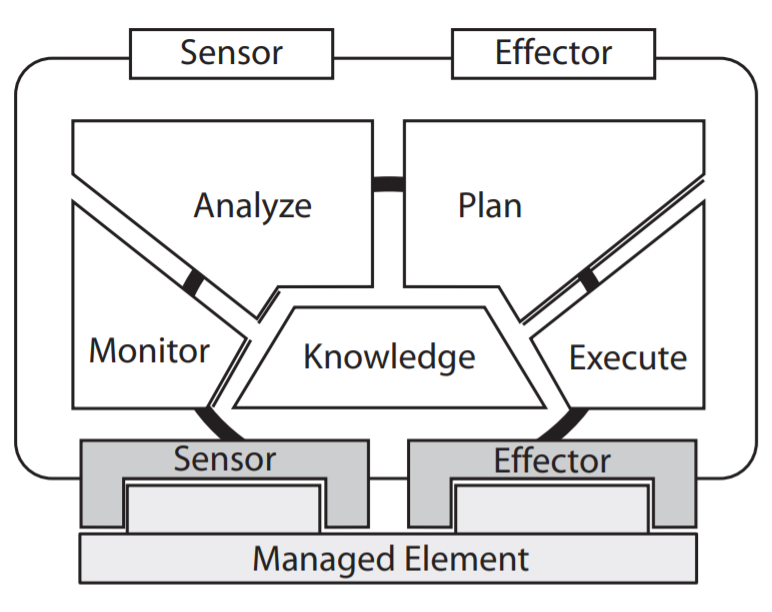
\includegraphics[scale=0.5]{images/MAPE-K.png}
\caption {Diagrama de funcionamento da arquitetura MAPE-K~\citep{Abbas_2010}.}
\label{fig:MAPEK}
\end{figure}

\section{Metodologia}

\subsection{Arquitetura}

Foi desenvolvido um sistema, cujo desenvolvimento pode ser dividido em 4 etapas principais:

\begin{itemize}
    \item {\textbf{Engenharia de dados:}} Etapa criada com o objetivo de simular processos de transformação e limpeza de dados.
    \item {\textbf{Workflow de IA:}} Etapa para execução de um Pipeline que simula o desenvolvimento de uma aplicação automatizada de IA, desde uma categorização dos dados mais específica do que na etapa anterior, passando pelo algoritmo utilizado e finalizando obtendo métricas para determinar qualidade do resultado final.
    \item {\textbf{Autonomia do Workflow (Componente MAPE-K):}} Etapa que executa um componente para automatizar todas as etapas do Workflow, com o objetivo de evitar com que perca-se tempo em execuções manuais que podem demorar dependendo do algoritimo e do conjunto de dados utilizado.
    \item {\textbf{Interface:}} Etapa criada com o objetivo de simular a etapa anterior, porém de modo a proporcionar uma experiência de usuário mais simples e intuitiva, onde sua integração com as outras etapas é mostrada na Figura \ref{fig:BackendFrontendML}. É dividida em duas partes:
    \begin{itemize}
        \item {\textbf{Frontend:}} Parte visual, exibida em um navegador.
        \item \textbf{{Backend:}} Parte onde o Frontend se comunica para obter os dados e montar o visual corretamente, de forma que corresponda a configurações utilizadas pelo Componente MAPE-K.
    \end{itemize}
\end{itemize}

\begin{figure}[H]
\centering
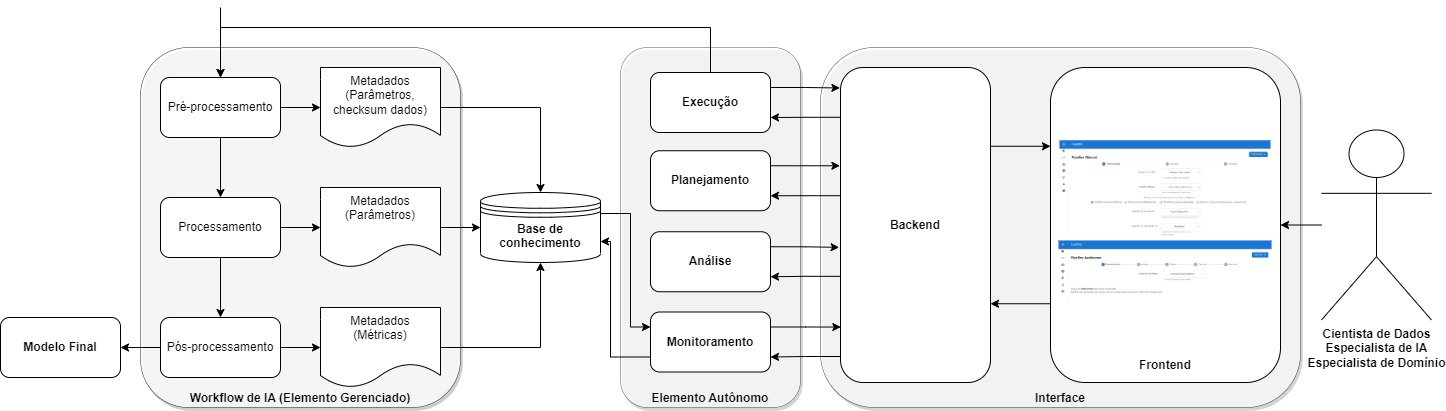
\includegraphics[scale=0.4]{images/backend-frontend-ml.jpg}
\caption {Comunicação entre Interface, autonomia e \textit{Workflow} de IA}
\label{fig:BackendFrontendML}
\end{figure}

Para o desenvolvimento do workflow, foi utilizada a arquitetura Pipe-and-Filter. Para a autonomia deste, foi criado um componente utilizando a arquitetura MAPE-K para analisar uma base de conhecimento e prover o melhor pipeline seguindo regras pré-determinadas. Para a interface, ela foi criada nos moldes de uma aplicação web. 

\subsection{Autonomia}

Para determinar a autonomia deste workflow, é realizado um cálculo de pesos baseado em uma seleção livre das métricas. O motivo de existir esse cálculo é mensurar o contexto do problema de acordo com uma análise prévia do Cientista de Dados e do Especialista de Domínio, e consolidar todas as métricas para simplificar as estratégias de planejamento. As métricas são divididas em dois grupos (Métricas de performance e Metricas de Fairness), e dentro desse grupo pode-se colocar quantas métricas forem necessárias, desde que seja respeitado o contexto de cada grupo. A cada grupo é atribuído pesos diferentes, e a cada métrica desse grupo também é atribuído pesos diferentes.

Primeiro, normaliza-se as métricas $m_{F_i}$ para $m'_{F_i}$, referentes às métricas de Fairness, para todas ficarem em um intervalo de 0 a 1, conforme exibido na equação \ref{eqn:normalizationFairness}. Dessa forma, seus resultados ficam uniformes e é possível aplicar os pesos sem haver distorções no cálculo. No caso das métricas de Performance, todas possuem a mesma escala, por isso as métricas $m_{P_i}$ não são normalizadas. Depois, multiplica-se cada uma por seus pesos correspondentes $w_{P_i}$ e $w_{F_i}$, e realiza-se uma média ponderada dentro do grupo para atribuir uma pontuação $S_P$ para o grupo das Métricas de Performance e $S_F$ para o grupo das Metricas de Fairness, conforme exibido na equação \ref{eqn:groupScores}. Para facilitar a visualização das pontuações, multiplica-se as pontuações por um fator $X = 1000$ para o intervalo da pontuação ser de 0 a 1000 e arredonda-se o número. Após tais pontuações serem obtidas, a pontuação geral $S$ é calculada multiplicando-as por seus pesos correspondentes $w_P$ e $w_F$ e realizando a média ponderada, conforme exibido na equação \ref{eqn:totalScore}.

\begin{equation}
\label{eqn:normalizationFairness}
	\begin{aligned}
	m'_{F_i} = 
	\begin{cases}
	1-\lvert m_{F_i} \rvert & \text{caso $m_{F_i}$ envolva diferen\c{c}a e $-1 < m_{F_i} < 1$}\\
	0 & \text{caso $m_{F_i}$ envolva diferen\c{c}a, e $m_{F_i} >= 1$ ou $m_{F_i} <= -1$}\\
	1-\lvert \frac{1}{m_{F_i}}-1 \lvert & \text{caso $m_{F_i}$ envolva razão e $m_{F_i} > 1$}\\
	1-\lvert m_{F_i}-1 \lvert & \text{caso $m_{F_i}$ envolva razão e $m_{F_i} <= 1$}\\
	m_{F_i} & \text{caso contrário}
	\end{cases}
	\end{aligned}
\end{equation}

\begin{equation}
\label{eqn:groupScores}
	\begin{aligned}
	S_F = \round{X \times \frac{\sum_{i=1}^{n_F} w_{m'_{F_i}} \times m'_{F_i}}{\sum_{i=1}^{n} w_{m'_{F_i}}}}\\
	S_P = \round{X \times \frac{\sum_{i=1}^{n_P} w_{m_{P_i}} \times m_{P_i}}{\sum_{i=1}^{n} w_{m_{P_i}}}}
	\end{aligned}
\end{equation}

\begin{equation}
\label{eqn:totalScore}
	S = \frac{w_F \times S_F + w_P \times S_P}{w_F + w_P}
\end{equation}

Para este cálculo ser realizado, é necessário como pré-requisito execuções anteriores realizadas no workflow, para que o mesmo grave as métricas necessárias e determine quais as melhores combinações através da pontuação.

\section{Estudos de Caso}

Foram realizados 3 Estudos de Caso para determinar a viabilidade de escolha das arquiteturas, manutenções futuras e funcionamento da autonomia na escolha de melhores \textit{Workflows} em diferentes contextos. Em todos eles, o objetivo foi a obtenção classificação de crédito (boa ou ruim), através de uma série de \textit{features}, mas utilizando diferentes conjuntos de dados. No caso de alterações no sistema, também foram contadas as linhas de código realizadas em cada alteração, para definir se tais alterações são simples de serem feitas.

A execução para determinar o melhor \textit{Workflow} foi realizada com 3 pesagens diferentes na pontuação geral:

\begin{itemize}
\item 50\% para métricas de Performance e 50\% para métricas de Fairness, para uma configuração equilibrada.
\item 75\% para métricas de Performance e 25\% para métricas de Fairness, para uma configuração que prioriza a performance em detrimento da justiça.
\item 25\% para métricas de Performance e 75\% para métricas de Fairness, para uma configuração que prioriza a justiça em detrimento da performance.
\end{itemize}

Em todas as execuções são utilizadas as métricas Acurácia, Precisão, \textit{Recall}, \textit{F1-Score} e AUC como métricas de Performance e as métricas \textit{Statistical Parity Difference}, \textit{Equal Opportunity Difference}, \textit{Average Odds Difference}, \textit{Disparate Impact} e \textit{Theil Index} como métricas de \textit{Fairness}, todas com pesagens iguais em seu respectivo agrupamento. Como não foram encontrados estudos onde são utilizados redução de viés em mais de uma parte do processo de Machine Learning (pré-processamento, processamento ou pós-processamento), é realizada a execução de apenas um algoritmo de redução de viés por \textit{workflow}.

\subsection{Viabilidade e utilidade do MAPE-K}

 Neste Estudo de Caso, o maior foco foi colocado em testar e verificar como o MAPE-K se comporta em um cenário com diversas execuções prévias de Workflows. Como as execuções geraram uma base de conhecimento, o componente MAPE-K pode executar uma análise através destes dados e determinar um plano indicando a gama de algoritmos que utilizará para obter melhores resultados, utilizando o German Credit Dataset~\citep{ucigerman_2021} como conjunto de dados. Os resultados estão presentes abaixo nas Tabelas \ref{tbl:ScoreMAPEKGeral5050}, \ref{tbl:ScoreMAPEKGeral7525} e \ref{tbl:ScoreMAPEKGeral2575}:

\begin{table}[H]
\begin{center}
  \caption{Melhores opções escolhidas pelo modelo MAPE-K \\ Todos os métodos - 50\% Performance/50\% Fairness}
\label{tbl:ScoreMAPEKGeral5050}
  \resizebox{\linewidth}{!}{%
\begin{tabular}{c|c|c|c|c|c|c}
\multicolumn{4}{c|}{Workflow} & \multicolumn{3}{c}{Pontuação} \\
\hline
Atributo protegido & Pré-processamento & Treinamento & Pós-processamento & Performance & Fairness & \textbf{Geral} \\
\hline
Idade & Nenhum & Regressão Logística & Equalized Odds & 968 & 860 & \textbf{914} \\
Nacionalidade & Nenhum & Random Forest & Calibrated Equalized Odds & 902 & 922 & \textbf{912} \\
Nacionalidade & Nenhum & Gradient Boosting & Calibrated Equalized Odds & 870 & 925 & \textbf{898} \\
Idade & Nenhum & Gradient Boosting & Equalized Odds & 927 & 862 & \textbf{894} \\
Idade & Reweighing & Gradient Boosting & Nenhum & 804 & 931 & \textbf{868} \\
\end{tabular}}
\end{center}
\end{table}

\begin{table}[H]
\begin{center}
  \caption{Melhores opções escolhidas pelo modelo MAPE-K \\ Todos os métodos - 75\% Performance/25\% Fairness}
\label{tbl:ScoreMAPEKGeral7525}
  \resizebox{\linewidth}{!}{%
\begin{tabular}{c|c|c|c|c|c|c}
\multicolumn{4}{c|}{Workflow} & \multicolumn{3}{c}{Pontuação} \\
\hline
Atributo protegido & Pré-processamento & Treinamento & Pós-processamento & Performance & Fairness & \textbf{Geral} \\
\hline
Idade & Nenhum & Regressão Logística & Equalized Odds & 968 & 860 & \textbf{941} \\
Idade & Nenhum & Gradient Boosting & Equalized Odds & 927 & 862 & \textbf{910} \\
Nacionalidade & Nenhum & Random Forest & Calibrated Equalized Odds & 902 & 922 & \textbf{907} \\
Nacionalidade & Nenhum & Gradient Boosting & Calibrated Equalized Odds & 870 & 925 & \textbf{883} \\
Idade & Nenhum & Random Forest & Equalized Odds & 898 & 799 & \textbf{874} \\
\end{tabular}}
\end{center}
\end{table}

\begin{table}[H]
\begin{center}
  \caption{Melhores opções escolhidas pelo modelo MAPE-K \\ Todos os métodos - 25\% Performance/75\% Fairness}
\label{tbl:ScoreMAPEKGeral2575}
  \resizebox{\linewidth}{!}{%
\begin{tabular}{c|c|c|c|c|c|c}
\multicolumn{4}{c|}{Workflow} & \multicolumn{3}{c}{Pontuação} \\
\hline
Atributo protegido & Pré-processamento & Treinamento & Pós-processamento & Performance & Fairness & \textbf{Geral} \\
\hline
Idade & Disparate Impact Remover & Support Vector Machines & Nenhum & 747 & 989 & \textbf{928} \\
Nacionalidade & Disparate Impact Remover & Support Vector Machines & Nenhum & 747 & 989 & \textbf{928} \\
Idade & Nenhum & Adversarial Debiasing & Nenhum & 742 & 979 & \textbf{920} \\
Nacionalidade & Reweighing & Support Vector Machines & Nenhum & 755 & 972 & \textbf{918} \\
Nacionalidade & Learning Fair Representations & Support Vector Machines & Nenhum & 755 & 972 & \textbf{918} \\
\end{tabular}}
\end{center}
\end{table}

Nessas execuções, surpreende 2 observações. A primeira é o fato da predominância de algoritmos com redução de viés no pós-processamento/resultado especialmente em configurações que priorizavam performance, contrariando o esperado de que os algoritmos com redução de viés aumentavam justiça em detrimento da performance. A segunda é a predominância de algoritmos com redução de viés no pré-processamento/dado em configurações que priorizavam justiça, principalmente pois todas as execuções usavam \textit{Support Vector Machines} como algoritmo de treinamento.

Diante destas 2 predominâncias envolvendo todos os \textit{workflows} executados, novos experimentos com restrições adicionais foram realizados para obter observações mais detalhadas a respeito dos resultados:

\begin{itemize}
\item Uso apenas de \textit{workflows} com o uso de algoritmos com redução de viés no pré - processamento/dado.
\item Uso apenas de \textit{workflows} com o uso de algoritmos com redução de viés no processamento/treinamento.
\item Uso apenas de \textit{workflows} com o uso de algoritmos com redução de viés no pós - processamento/resultado.
\item Uso apenas de \textit{workflows} sem o uso de algoritmos com redução de viés.
\end{itemize}

Nos \textit{workflows} utilizando apenas algoritmos com redução de viés no dado, percebe-se a predominância dos algoritmos de treinamento \textit{Gradient Boosting} e \textit{Support Vector Machines}, sendo o \textit{Gradient Boosting} predominante em configurações priorizando performance e o \textit{Support Vector Machines} predominante em configurações priorizando justiça, o que começa a explicar a sua predominância também presente no resultado geral. Também é possível perceber mais 2 observações: A primeira observação é que a análise de apenas uma categoria de algoritmos dá mais clareza em ver como o cálculo utilizado nas 3 configurações faz com que o equilíbrio de ambas as métricas se torna mais importante do que a prioridade apenas em performance ou apenas em justiça, uma vez que há exemplos de conjuntos de algoritmos com pontuações ligeiramente maiores em performance que acabaram sendo pior avaliados pois a pontuação em \textit{Fairness} está bem menor, e vice-versa. A segunda observação é que o uso de um atributo protegido diferente (e, por consequência, com tratamento de dados diferente) e de um algoritmo de treinamento parecem impactar tanto quanto ou até mais que o próprio algoritmo com redução de viés no dado.

Nos \textit{workflows} utilizando apenas algoritmos com redução de viés no treinamento, percebe-se uma variedade maior nos algoritmos, até porque não há usos de redução de viés em um pré ou um pós-processamento, com destaque para o \textit{Adversarial Debiasing} que foi bem avaliado pela pontuação alta em \textit{Fairness}. Nestes \textit{workflows}, as 2 observações percebidas nos \textit{workflows} utilizando apenas algoritmos com redução de viés no dado são reforçadas por uma maior variedade de pontuações e pelo algoritmo \textit{Exponentiated Gradient Reduction} com 2 exemplos diferentes na Tabela \ref{tbl:ScoreMAPEKInproc7525}, onde o uso da Nacionalidade como atributo protegido possui pontuações de performance e \textit{Fairness} piores que a Idade e conclundo que o processamento utilizado no atributo protegido pode afetar todas as métricas.

Nos \textit{workflows} utilizando apenas algoritmos com redução de viés no resultado, surpreende o fato de que os \textit{workflows} obtiveram as melhores pontuações em Performance e as piores pontuações em \textit{Fairness}, podendo indicar uma característica dos algoritmos \textit{Equalized Odds} e \textit{Calibrated Equalized Odds}. Entretanto, por conta da grande melhora por parte das métricas de performance, estes \textit{workflows} possuem um maior equilíbrio entre Performance e \textit{Fairness} e acabam garantindo maiores pontuações na média, justificando as melhores pontuações nas primeiras execuções onde foram considerados todos os métodos. Fora isto, as demais observações anteriores também se aplicam nestas execuções.

Nos \textit{workflows} sem algoritmos com redução de viés, é curioso notar que, ao comparar com \textit{workflows} equivalentes mas com algoritmos usando redução de viés no dado, é possível notar que a hipótese principal se confirma em sua grande maioria: As pontuações em Performance são ligeiramente maiores e as pontuações em \textit{Fairness} são ligeiramente menores. É possível notar uma exceção no \textit{workflow} envolvendo o algoritmo \textit{Random Forest}, mas nos outros casos a hipótese é verificada com sucesso. Ao comparar com \textit{workflows} usando algoritmos com redução de viés no treinamento tal hipótese também se confirma, entretanto o uso de \textit{Support Vector Machines} parece ser uma exceção a regra, implicando que o uso do algoritmo possibilita modelos mais justos para o conjunto de dados utilizado. Ao comparar com \textit{workflows} usando algoritmos com redução de viés no resultado, a hipótese não se confirma devido a observação da grande melhora por parte das métricas de performance nos \textit{workflows} usando algoritmos com redução de viés no resultado, mas ao verificar a pontuação em \textit{Fairness} é possível notar uma ligeira melhora. Há a exceção de \textit{workflows} envolvendo \textit{Support Vector Machines} que são melhores nos \textit{workflows} sem algoritmos com redução de viés, mas no uso de outros algoritmos ocorre melhora na pontuação em \textit{Fairness}.

Em todas as execuções, foi possível perceber que a escolha do \textit{workflow} com o melhor equilíbrio entre estes dois grupos de métricas com contextos completamente diferentes ainda se torna difuso diante da grande quantidade de métricas e conjuntos de algoritmos utilizados. Além disso, a diferença entre as métricas é extremamente pequena e dificulta ainda mais a escolha. Nesse contexto, a consolidação das métricas em grupos simplifica a visualização de quais \textit{workflows} são mais equilibrados, e o uso de pesos para cada métrica e para cada grupo pode calibrar qual o melhor equilíbrio desejado para determinada situação. Deste modo, pode-se concluir também que, em um contexto de desenvolvimento, o processo simplifica a decisão do Cientista de Dados e reduz significantemente o tempo para obtenção e implantação de um modelo otimizado, pois não exigirá execuções em diversos algoritmos uma vez que já há uma base de conhecimento prévia. Além disso, poderá poupar processamento e custos para a resolução de diversos outros problemas, uma vez que as execuções economizadas pelas equipes que utilizariam esse processo abrem margem para que outras equipes utilizem esse processamento.

\subsection{Evolução do \textit{Workflow} adicionando um novo conjunto de dados}

Neste Estudo de Caso, foi realizada uma evolução do sistema adicionando um novo conjunto de dados mais próximo de conjuntos de dados reais. Além de reforçar a versatilidade do MAPE-K em diferentes contextos, um maior foco foi colocado na manutenção do sistema, discutindo se as etapas e arquiteturas escolhidas são viáveis para evoluir e manter o \textit{Workflow} sem grandes deteriorações nas ideias originais de seu desenvolvimento, desta vez utilizando o Lendingclub Dataset~\citep{lendingclub_2022} como conjunto de dados. Os resultados estão presentes abaixo nas Tabelas \ref{tbl:ScoreMAPEKLendingclubGeral5050}, \ref{tbl:ScoreMAPEKLendingclubGeral7525} e \ref{tbl:ScoreMAPEKLendingclubGeral2575}:

\begin{table}[H]
\begin{center}
  \caption{Melhores opções escolhidas pelo modelo MAPE-K \\ Todos os métodos - 50\% Performance/50\% Fairness}
\label{tbl:ScoreMAPEKLendingclubGeral5050}
  \resizebox{\linewidth}{!}{%
\begin{tabular}{c|c|c|c|c|c|c}
\multicolumn{4}{c|}{Workflow} & \multicolumn{3}{c}{Pontuação} \\
\hline
Atributo protegido & Pré-processamento & Treinamento & Pós-processamento & Performance & Fairness & \textbf{Geral} \\
\hline
Renda & Learning Fair Representations & Random Forest & Nenhum & 991 & 968 & \textbf{979} \\
Renda & Nenhum & Gradient Boosting & Equalized Odds & 988 & 969 & \textbf{978} \\
Renda & Reweighing & Random Forest & Nenhum & 991 & 963 & \textbf{977} \\
Renda & Learning Fair Representations & Regressão Logística & Nenhum & 981 & 973 & \textbf{977} \\
Renda & Reweighing & Gradient Boosting & Nenhum & 987 & 964 & \textbf{976} \\
\end{tabular}}
\end{center}
\end{table}

\begin{table}[H]
\begin{center}
  \caption{Melhores opções escolhidas pelo modelo MAPE-K \\ Todos os métodos - 75\% Performance/25\% Fairness}
\label{tbl:ScoreMAPEKLendingclubGeral7525}
  \resizebox{\linewidth}{!}{%
\begin{tabular}{c|c|c|c|c|c|c}
\multicolumn{4}{c|}{Workflow} & \multicolumn{3}{c}{Pontuação} \\
\hline
Atributo protegido & Pré-processamento & Treinamento & Pós-processamento & Performance & Fairness & \textbf{Geral} \\
\hline
Renda & Nenhum & Regressão Logística & Equalized Odds & 985 & 965 & \textbf{980} \\
Renda & Learning Fair Representations & Gradient Boosting & Nenhum & 987 & 960 & \textbf{980} \\
Renda & Learning Fair Representations & Regressão Logística & Nenhum & 981 & 973 & \textbf{979} \\
Renda & Nenhum & Grid Search Reduction & Nenhum & 989 & 950 & \textbf{979} \\
Renda & Reweighing & Regressão Logística & Nenhum & 981 & 965 & \textbf{977} \\
\end{tabular}}
\end{center}
\end{table}

\begin{table}[H]
\begin{center}
  \caption{Melhores opções escolhidas pelo modelo MAPE-K \\ Todos os métodos - 25\% Performance/75\% Fairness}
\label{tbl:ScoreMAPEKLendingclubGeral2575}
  \resizebox{\linewidth}{!}{%
\begin{tabular}{c|c|c|c|c|c|c}
\multicolumn{4}{c|}{Workflow} & \multicolumn{3}{c}{Pontuação} \\
\hline
Atributo protegido & Pré-processamento & Treinamento & Pós-processamento & Performance & Fairness & \textbf{Geral} \\
\hline
Renda & Learning Fair Representations & Regressão Logística & Nenhum & 981 & 973 & \textbf{975} \\
Renda & Nenhum & Gradient Boosting & Equalized Odds & 988 & 969 & \textbf{974} \\
Renda & Learning Fair Representations & Random Forest & Nenhum & 991 & 968 & \textbf{973} \\
Renda & Nenhum & Exponentiated Gradient Reduction & Nenhum & 986 & 966 & \textbf{971} \\
Renda & Reweighing & Gradient Boosting & Nenhum & 987 & 964 & \textbf{970} \\
\end{tabular}}
\end{center}
\end{table}

Nessas execuções, a principal observação notada é que a relação de algoritmos com melhores desempenhos mudou completamente, com predominância do algoritmo \textit{Learning Fair Representations} para redução de viés e Regressão Logística para algoritmo de treinamento. Também se nota que algoritmos com redução de viés no pós-processamento e algoritmos de treinamento como \textit{Support Vector Machines} não foram tão eficientes. Com isso, pode-se concluir que, ao mudar o contexto do problema e os dados envolvidos, o MAPE-K pode ajudar a enxergar tais sutilezas e ajudar em uma decisão de forma mais eficiente e ágil. Entretanto, os dados e metadados obtidos não ajudaram a entender o porquê de tais sutilezas acontecerem.

Para processar o Lendingclub Dataset, foram necessárias modificações para realizar a evolução do sistema e adicionar este conjunto de dados como opção no \textit{Workflow}. Estas foram contadas de acordo com seus \textit{commits} realizados no repositório e exibidos  na Tabela \ref{tbl:ManutencaoPipelineDataset}:

\begin{table}[H]
\begin{center}
  \caption{Quantidade de modificações realizadas ao adicionar um novo conjunto de dados ao \textit{Workflow}}
\label{tbl:ManutencaoPipelineDataset}
  \resizebox{\linewidth}{!}{%
{\def\arraystretch{1.5}
\begin{tabular}{c|c|c|c|c|c|c}
Parte do Sistema & \makecell{Linhas alteradas} & Total de linhas & \makecell{Arquivos alterados} & Total de arquivos & \makecell{\% linhas alteradas} & \makecell{\% arquivos alterados} \\
\hline
\makecell{Engenharia de Dados} & 122 & 277 & 2 & 3 & \textbf{44,04\%} & \textbf{66,67\%} \\
\textit{Workflow} de IA & 76 & 1982 & 5 & 38 & \textbf{3,84\%} & \textbf{13,16\%} \\
Autonomia do \textit{Workflow} & 0 & 457 & 0 & 10 & \textbf{0,00\%} & \textbf{0,00\%} \\
\makecell{Interface Humano-Computador (\textit{Frontend})} & 13 & 2905 & 2 & 14 & \textbf{0,45\%} & \textbf{14,29\%} \\
\makecell{Interface Humano-Computador (\textit{Backend})} & 4 & 432 & 1 & 7 & \textbf{0,93\%} & \textbf{14,29\%} \\
\hline
\textbf{TOTAL} & \textbf{215} & \textbf{6053} & \textbf{10} & \textbf{72} & \textbf{3,55\%} & \textbf{13,89\%} \\
\end{tabular}}}
\end{center}
\end{table}

A adição do conjunto de dados não exigiu modificações no Componente MAPE-K, mesmo os resultados sendo completamente diferentes do Estudo de Caso anterior. Isto reforça a autonomia proposta no MAPE-K, possibilitando escolhas diferentes baseadas nos metadados presentes no \textit{Workflow} sem realizar modificações. O Componente MAPE-K só exigirá modificações se os metadados salvos do \textit{Workflow} forem modificados, ou se modificar alguma configuração intrínseca ao próprio MAPE-K, que não possui nenhuma relação com o \textit{Workflow}. 

Os elementos na Interface Humano-Computador exigiram pouquíssimas modificações, podendo ser resumidos a simples adições para colocar a opção do novo conjunto de dados. As maiores modificações foram realizadas no \textit{Workflow} de IA e nas Transformações do Conjunto de Dados, principalmente deste último. Das modificações no \textit{Workflow} de IA, a grande parte (34 linhas, ou 44,74\% das linhas) foi realizada no pré-processamento do dado para o cálculo dos algoritmos de treinamento. Embora a estruturação baseada na arquitetura \textit{Pipe-and-Filter} traga algumas linhas a mais para as modificações devido a quantidade de classes criadas para o \textit{workflow} (2 para pipes e 1 para filtro), etapas de processamento e transformação dos dados serão as partes de onde se consumirá mais tempo e modificações por parte dos Engenheiros e Cientistas de Dados.

Embora tenha a consequência de escrever algumas linhas a mais, o uso da arquitetura \textit{Pipe-and-Filter} permite o encapsulamento dos algoritmos e a separação de interesses de forma simples, fazendo com que a parte de código existente para o \textit{workflow} possa ter escolhas mais interessantes e elegantes para um bom \textit{Design} do código. Dito isso, realizar a manutenção/evolução do sistema no \textit{Workflow} e na Interface Humano-Computador é relativamente simples, desde que se saiba os arquivos onde as modificações serão realizadas. Por isso, a criação de uma documentação é extremamente importante para que um novo desenvolvedor entenda o todo do sistema e não adicione linhas em trechos desnecessários.

\subsection{Evolução do \textit{Workflow} com desenvolvedor sem conhecimento anterior adicionando um novo algoritmo de treinamento}

Neste Estudo de Caso, foi realizada uma evolução do sistema adicionando um novo algoritmo de classificação. O foco ainda é na manutenção do sistema, mas desta vez foi colocado para outros desenvolvedores desenvolverem a solução. A discussão se focará mais se as arquiteturas escolhidas são versáteis e simples o suficiente para que pessoas entendam o contexto do sistema e façam novas evoluções, novamente utilizando o Lendingclub Dataset~\citep{lendingclub_2022} como conjunto de dados. 

Foi realizada uma sessão de desenvolvimento com um outro desenvolvedor, durando um tempo entre 1 e 2 horas, onde este adicionou um novo algoritmo de classificação dentro da estrutura do \textit{workflow} com a documentação montada durante o Estudo de caso anterior. Durante a sessão, alguns itens como erros na documentação e bugs foram notados e corrigidos, através de observação e \textit{feedbacks} do desenvolvedor. Por causa destes erros, uma pequena parte da sessão foi gasto em auxílios e dúvidas para que o desenvolvedor pudesse realizar o desenvolvimento sem que precisasse gastar o tempo identificando problemas que não foram de responsabilidade dele. Depois da sessão, o desenvolvedor preencheu um questionário, refletindo um perfil com certa experiência na área de dados e desenvolvimento. No geral, as impressões foram positivas e a implementação ocorreu sem dificuldades. Embora a intenção inicial era que o desenvolvedor apenas se guiasse pela documentação e o auxílio durante a sessão acabou facilitado o entendimento por parte do desenvolvedor, ele próprio considerou a adaptação a tal experimento rápida. Dada a afirmação, é possível concluir que as decisões arquiteturais tomadas foram corretas e facilitaram o desenvolvimento de evoluções.

O algoritmo de classificação escolhido para o desenvolvimento foi o Naive Bayes~\citep{Naive_Bayes_2004}, que também é bastante difundido como classificador. Após o desenvolvimento, os resultados baseados nas pré-condições e restrições já comentadas na seção anterior estão presentes abaixo nas Tabelas \ref{tbl:ScoreMAPEKLendingclubCaso35050}, \ref{tbl:ScoreMAPEKLendingclubCaso37525} e \ref{tbl:ScoreMAPEKLendingclubCaso32575}:

\begin{table}[H]
\begin{center}
  \caption{Melhores opções escolhidas pelo modelo MAPE-K \\ Todos os métodos - 50\% Performance/50\% Fairness}
\label{tbl:ScoreMAPEKLendingclubCaso35050}
  \resizebox{\linewidth}{!}{%
\begin{tabular}{c|c|c|c|c|c|c}
\multicolumn{4}{c|}{Workflow} & \multicolumn{3}{c}{Pontuação} \\
\hline
Atributo protegido & Pré-processamento & Treinamento & Pós-processamento & Performance & Fairness & \textbf{Geral} \\
\hline
Renda & Learning Fair Representations & Random Forest & Nenhum & 991 & 968 & \textbf{979} \\
Renda & Nenhum & Gradient Boosting & Equalized Odds & 988 & 969 & \textbf{978} \\
Renda & Reweighing & Random Forest & Nenhum & 991 & 963 & \textbf{977} \\
Renda & Learning Fair Representations & Regressão Logística & Nenhum & 981 & 973 & \textbf{977} \\
Renda & Reweighing & Gradient Boosting & Nenhum & 987 & 964 & \textbf{976} \\
\end{tabular}}
\end{center}
\end{table}

\begin{table}[H]
\begin{center}
  \caption{Melhores opções escolhidas pelo modelo MAPE-K \\ Todos os métodos - 75\% Performance/25\% Fairness}
\label{tbl:ScoreMAPEKLendingclubCaso37525}
  \resizebox{\linewidth}{!}{%
\begin{tabular}{c|c|c|c|c|c|c}
\multicolumn{4}{c|}{Workflow} & \multicolumn{3}{c}{Pontuação} \\
\hline
Atributo protegido & Pré-processamento & Treinamento & Pós-processamento & Performance & Fairness & \textbf{Geral} \\
\hline
Renda & Nenhum & Regressão Logística & Equalized Odds & 985 & 965 & \textbf{980} \\
Renda & Learning Fair Representations & Gradient Boosting & Nenhum & 987 & 960 & \textbf{980} \\
Renda & Learning Fair Representations & Regressão Logística & Nenhum & 981 & 973 & \textbf{979} \\
Renda & Nenhum & Grid Search Reduction & Nenhum & 989 & 950 & \textbf{979} \\
Renda & Reweighing & Regressão Logística & Nenhum & 981 & 965 & \textbf{977} \\
\end{tabular}}
\end{center}
\end{table}

\begin{table}[H]
\begin{center}
  \caption{Melhores opções escolhidas pelo modelo MAPE-K \\ Todos os métodos - 25\% Performance/75\% Fairness}
\label{tbl:ScoreMAPEKLendingclubCaso32575}
  \resizebox{\linewidth}{!}{%
\begin{tabular}{c|c|c|c|c|c|c}
\multicolumn{4}{c|}{Workflow} & \multicolumn{3}{c}{Pontuação} \\
\hline
Atributo protegido & Pré-processamento & Treinamento & Pós-processamento & Performance & Fairness & \textbf{Geral} \\
\hline
Renda & Nenhum & Naive Bayes & Calibrated Equalized Odds & 991 & 976 & \textbf{980} \\
Renda & Learning Fair Representations & Regressão Logística & Nenhum & 981 & 973 & \textbf{975} \\
Renda & Nenhum & Gradient Boosting & Equalized Odds & 988 & 969 & \textbf{974} \\
Renda & Learning Fair Representations & Random Forest & Nenhum & 991 & 968 & \textbf{973} \\
Renda & Nenhum & Exponentiated Gradient Reduction & Nenhum & 986 & 966 & \textbf{971} \\
\end{tabular}}
\end{center}
\end{table}

Para o contexto do Lendingclub Dataset a adição do Naive Bayes no \textit{workflow} mostrou seu valor, apresentando uma pontuação acima do esperado para configurações que privilegiam justiça e só não foi mais destacada por causa do limiar máximo estabelecido de 980. Entretanto, como já visto em estudos de caso anteriores, pode não funcionar em outros contextos e os dados e metadados estabelecidos não definem explicações do porquê o Naive Bayes teve um comportamento positivo para este conjunto de dados.

As evoluções realizadas no \textit{Workflow} para adicionar o Naive Bayes foram contadas de acordo com seus \textit{commits} realizados no repositório e exibidos  na Tabela \ref{tbl:ManutencaoPipelineDataset}:

\begin{table}[H]
\begin{center}
  \caption{Quantidade de modificações realizadas ao adicionar um novo algoritmo ao \textit{Workflow}}
\label{tbl:ManutencaoPipelineCaso3}
  \resizebox{\linewidth}{!}{%
{\def\arraystretch{1.5}
\begin{tabular}{c|c|c|c|c|c|c}
Parte do Sistema & \makecell{Linhas alteradas} & Total de linhas & \makecell{Arquivos alterados} & Total de arquivos & \makecell{\% linhas alteradas} & \makecell{\% arquivos alterados} \\
\hline
\makecell{Engenharia de Dados} & 0 & 277 & 0 & 3 & \textbf{0,00\%} & \textbf{0,00\%} \\
\textit{Workflow} de IA & 60 & 2042 & 5 & 39 & \textbf{2,94\%} & \textbf{12,82\%} \\
Autonomia do \textit{Workflow} & 1 & 458 & 1 & 10 & \textbf{0,22\%} & \textbf{10,00\%} \\
\makecell{Interface Humano-Computador (\textit{Frontend})} & 71 & 2948 & 3 & 14 & \textbf{2,41\%} & \textbf{21,43\%} \\
\makecell{Interface Humano-Computador (\textit{Backend})} & 1 & 433 & 1 & 7 & \textbf{0,23\%} & \textbf{14,29\%} \\
\hline
\textbf{TOTAL} & \textbf{132} & \textbf{6157} & \textbf{9} & \textbf{72} & \textbf{2,14\%} & \textbf{12,50\%} \\
\end{tabular}}}
\end{center}
\end{table}

Desta vez, a única parte do sistema sem necessidade de modificações foi a parte de Transformação do conjunto de dados. Entretanto, a única modificação necessária no componente MAPE-K e no \textit{Backend} da Interface Humano-Computador foi a adição do Naive Bayes como parte de uma parametrização, que poderia ser transferida para um arquivo externo de configuração e não exigir modificações futuramente.

No geral, foram exigidas menos modificações que a evolução proposta no Estudo de Caso anterior. A única parte que exigiu mais modificações foi no \textit{Frontend} da Interface Humano-Computador, em grande parte por causa de um único componente presente na tela de Configurações para Planejamento do MAPE-K. Fora esta exceção, adicionar um algoritmo é uma evolução mais simples de ser feita, e junto com a documentação criada um desenvolvedor com relativa experiência consegue executar essa tarefa sem grandes dificuldades.

\section{Conclusões e Trabalhos Futuros}

Pode-se dizer que o conjunto da arquitetura de \textit{Pipe-And-Filter} com a arquitetura MAPE-K se adaptou muito bem na implementação dos objetivos principais. Com a arquitetura \textit{Pipe-And-Filter}, foi possível encapsular todos os procedimentos presentes em um \textit{workflow} de uma aplicação de IA em etapas coesas e trocá-las caso haja a necessidade de teste com outro algoritmo, atributo protegido ou conjunto de dados. Com a proveniência dos dados, presente durante a avaliação dos modelos no \textit{workflow}, foi possível coletar os dados e métricas para a elaboração de uma Base de Conhecimento. Com a arquitetura MAPE-K, foi possível realizar um fluxo para que os dados obtidos no processo fossem filtrados, analisados para que haja uma tomada de decisão automática. Com a junção destes três conceitos, foi possível estabelecer um \textit{workflow} automatizado, dependendo apenas dos próprios dados obtidos em execuções anteriores para a automação ser executada. Entretanto, pode-se notar alguns pontos na implementação que não irão ser resolvidos apenas pela escolha da arquitetura.

Embora o \textit{Pipe-And-Filter} seja um modelo que facilite o encapsulamento e a segmentação dos procedimentos do \textit{workflow}, ele ainda é preso a limitações de fatores externos ao código, como o Hardware de onde será rodado e os dados a serem trabalhados. Desse modo, ao realizar a implementação, quem desenvolve terá de escolher um equilíbrio entre memória, armazenamento e performance. Por exemplo, como neste projeto os conjuntos de dados avaliados eram pequenos, eles puderam ser armazenados em memória e garantir performance máxima, mas conforme o número de dados avaliados for crescendo é necessário sacrificar performance e realizar as operações em dispositivos de armazenamento para manter a aplicação estável e com o mesmo custo, não necessitando da contratação de mais desenvolvedores e evitando gastos com infra-estrutura.

Embora olhar para a proveniência dos dados permita o armazenamento de dados importantes para estabelecer um elo entre o \textit{workflow} e o componente MAPE-K, não foi possível garantir que ela substitua Explainable AI pois não foram encontradas evidências do porquê de determinados algoritmos funcionarem em determinados conjuntos de dados e não em outros com os metadados cadastrados na base de conhecimento. A qualidade dos dados também é um ponto que deverá ser observado conforme o número de dados for crescente: É possível ter resultados fora do comum (\textit{outliers}), alguns atributos podem não permitir uma avaliação acurada, ou a quantidade de atributos pode não ser suficiente para avaliar. Antes da proveniência ser implementada, os próprios dados precisam ser modelados conforme o problema exige. Após a implementação, é preciso realizar processos de limpeza dos dados conforme execuções no \textit{workflow} vão sendo realizadas.

Embora o MAPE-K permita o desenvolvimento de uma aplicação autônoma, isso não significa que ela seja seja completamente automatizada para qualquer problema relacionado a \textit{Machine Learning}, necessitando de ação humana para funcionar. A principal limitação por parte do desenvolvimento é que a biblioteca AIF360 suporta apenas problemas de classificação binária, e para evoluções e novos métodos é provável que ocorram refatorações no \textit{workflow}. Também há de se considerar que, mesmo que o \textit{workflow} evolua para abrigar outros tipos de problemas, o contexto do problema é importante ao se avaliar se o modelo é considerado bom ou não. O uso de pesos para as métricas e diferentes estratégias nas fases de análise e planejamento do MAPE-K ajudam a definir o contexto para uma avaliação, mas ainda vai depender de um Cientista de Dados e/ou de um especialista de Domínio para entender quais as necessidades do problema analisado e se os resultados são aceitáveis para a publicação de um modelo otimizado.

% As referências:
\bibliographystyle{plainnat}
\bibliography{full,article}

\end{document}
